\documentclass{beamer}
\usetheme{default}
\usepackage{xcolor, colortbl}
\usepackage{algorithm}
\usepackage{algpseudocode}
\usepackage{textcomp}
\usepackage{listings}
\usepackage{hyperref}
\usepackage{alltt}
\usepackage{tikz}
\usepackage{framed}
\usepackage{marvosym}
\usepackage{wasysym}
\usepackage{marvosym}
\usepackage{crayola}
\usepackage{mathpartir}
\usepackage{tabularx}
\usepackage[belowskip=-15pt,aboveskip=0pt]{caption}
\usepackage[skins]{tcolorbox}
\usepackage{multicol}
\usetikzlibrary{positioning,shapes,arrows, arrows.meta, backgrounds, fit, shadows, automata}
\usetikzlibrary{decorations.markings, calc}
%\usepackage{wasysym}
%\usepackage{marvosym}
\setbeamertemplate{footline}[frame number]
%\usecolortheme{fly}
\usefonttheme{serif}

\title[Sujit]{Flowcharts}
\author{Sujit Kumar Chakrabarti}
\institute{}
\date{}

\definecolor{lightblue}{rgb}{0.8,0.93,1.0} % color values Red, Green, Blue
\definecolor{darkblue}{rgb}{0.4,0.3,1.0} % color values Red, Green, Blue
\definecolor{Blue}{rgb}{0,0,1.0} % color values Red, Green, Blue
\definecolor{darkgreen}{rgb}{0,0.7,0.2} % color values Red, Green, Blue
\definecolor{Red}{rgb}{1,0,0} % color values Red, Green, Blue
\definecolor{Pink}{rgb}{0.7,0,0.2}
\definecolor{links}{HTML}{2A1B81}
\definecolor{mydarkgreen}{HTML}{126215}
\newcommand{\highlight}[1]{{\color{Red}(#1)}}

\newcommand{\myheader}[1]{
	{\color{darkblue}
		\begin{Large}
			\begin{center}
				{#1}
			\end{center}
		\end{Large}
	}
}
\newcommand{\myminorheader}[1]{
	{\color{BrickRed}
		\begin{Large}
			{\fontfamily{\sfdefault}\selectfont\textbf{#1}}
		\end{Large}
	}
}


\tikzstyle{bb}=[%
      rectangle, draw=black, thick, fill=OliveGreen!30, drop shadow, align=center,
      text ragged, minimum height=2em, minimum width=2em, inner sep=6pt
]

\tikzstyle{inv}=[%
      rectangle, draw=none,  align=center,
      text ragged, minimum height=2em, minimum width=2em, align=center, inner sep=6pt
]

\tikzstyle{db}=[%
      diamond, draw=black, thick, fill=pink, drop shadow, align=center,
      text ragged, minimum height=2em, inner sep=6pt
]

\tikzstyle{jn}=[%
      inner sep=0cm, outer sep=0cm
]

\tikzstyle{io}=[%
      trapezium, trapezium left angle=60, trapezium right angle=120, draw=black, thick, fill=brown, drop shadow,
      text ragged, minimum height=2em, minimum width=2em, inner sep=6pt, align=center
]

\tikzstyle{glio}=[%
      trapezium, trapezium left angle=60, trapezium right angle=120, draw=red, line width = 1mm, fill=brown, drop shadow,
      text ragged, minimum height=2em, minimum width=2em, inner sep=6pt
]
\tikzstyle{gl}=[%
      rectangle, draw=red, line width = 1mm, fill=lightblue, drop shadow,
      text ragged, minimum height=2em, minimum width=2em, inner sep=6pt
]

\tikzstyle{en}=[%
      rectangle, draw=black, thick, fill=none,
      text ragged, minimum height=2em, minimum width=2em, inner sep=6pt
]


\tikzstyle{st}=[%
      ellipse, draw=Black, fill=Gray!20,
      text ragged, minimum height=2em, minimum width=2em, inner sep=6pt
]

\tikzstyle{kcedge}=[%
      -{Latex[length=3mm,width=2mm]}, Red, thick
]


\lstdefinestyle{javacode}{
	language = Java,
	basicstyle = \ttfamily\scriptsize,
	stringstyle = \ttfamily,
	keywordstyle=\color{Blue}\bfseries,
	identifierstyle=\color{Pink},
	commentstyle=\color{darkgreen},
	frame=single,
	frameround=tttt,
%	numbers=left
	showstringspaces=false
}

\lstdefinestyle{camlcode}{
	language = Caml,
	basicstyle = \scriptsize\ttfamily,
	stringstyle = \color{red}\ttfamily,
	keywordstyle=\color{Blue}\bfseries,
	identifierstyle=\ttfamily,
	frame=single,
	frameround=tttt,
	numbers=none,
	showstringspaces=false,
	escapeinside={(*@}{@*)}
}

\lstdefinestyle{outputcode}{
	language = bash,
	backgroundcolor = \color{black},
	basicstyle = \tiny\ttfamily\color{white},
	stringstyle = \color{red}\ttfamily,
	keywordstyle=\color{white}\bfseries,
	identifierstyle=\ttfamily,
	frameround=tttt,
	numbers=none,
	showstringspaces=false,
	escapeinside={(*@}{@*)}
}

\newtcolorbox{myframe}[2][]{%
  enhanced,colback=white,colframe=black,coltitle=black,
  sharp corners,boxrule=0.4pt,
  fonttitle=\itshape,
  attach boxed title to top left={yshift=-0.3\baselineskip-0.4pt,xshift=2mm},
  boxed title style={tile,size=minimal,left=0.5mm,right=0.5mm,
    colback=white,before upper=\strut},
  title=#2,#1
}

\begin{document}
\maketitle

\newcounter{qnum}
\addtocounter{qnum}{1}
% frame begin %%%%%%%%%%%%%%%%%%%%%%%%
\begin{frame}[fragile]{Flowchart}
{Sequence of Instructions}
\textbf{PROBLEM \theqnum:} You are in front of the door of your house. The door is already locked. Enter the house and lock the door from inside.
\begin{center}
\begin{tabular}{c @{} c}
\begin{minipage}{0.45\textwidth}
\begin{lstlisting}
Unlock door
Open door
Walk into house
Shut door
Lock door
\end{lstlisting}
\end{minipage}
&
\begin{minipage}{0.45\textwidth}
\pause
\begin{center}
\resizebox{!}{0.6\textheight}{
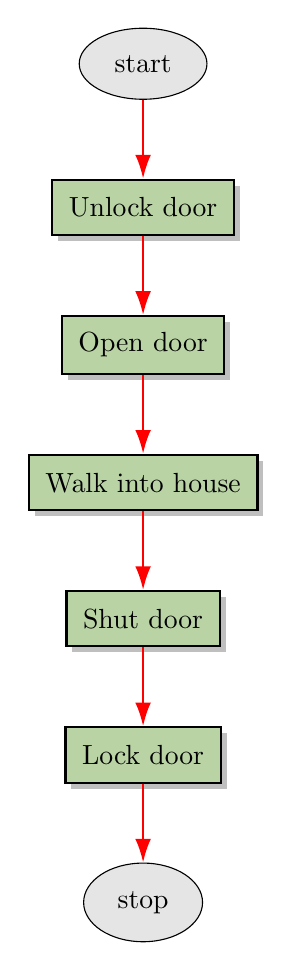
\begin{tikzpicture}[auto,
    -{Latex[length=3mm,width=2mm]},
    >=stealth
  ]
\node[st](start) {start};
\node[bb, below=of start](1) {Unlock door};
\node[bb, below= of 1](2) {Open door};
\node[bb, below= of 2](3) {Walk into house};
\node[bb, below= of 3](4) {Shut door};
\node[bb, below= of 4](5) {Lock door};
\node[st, below=of 5](stop) {stop};

\draw[kcedge] (start) to (1);
\draw[kcedge] (1) to (2);
\draw[kcedge] (2) to (3);
\draw[kcedge] (3) to (4);
\draw[kcedge] (4) to (5);
\draw[kcedge] (5) to (stop);
  \end{tikzpicture}
}
\end{center}

\end{minipage}

\end{tabular}
\end{center}

\end{frame}
% frame end %%%%%%%%%%%%%%%%%%%%%%%%

\addtocounter{qnum}{1}
% frame begin %%%%%%%%%%%%%%%%%%%%%%%%
\begin{frame}[fragile]{Flowchart}
{If branch}
\textbf{PROBLEM \theqnum:} You are in front of the door of your house. It is not known earlier if the door is locked or not. Enter the house and lock the door from inside. 

\begin{center}
\begin{tabular}{c @{} c}
\begin{minipage}{0.45\textwidth}
\begin{lstlisting}[basicstyle=\ttfamily\scriptsize]
Check if the door is locked
 or not
IF the check succeeds THEN DO 
  Unlock door
ENDIF
\end{lstlisting}
\end{minipage}
&
\begin{minipage}{0.45\textwidth}
\pause
\begin{center}
\resizebox{!}{0.6\textheight}{
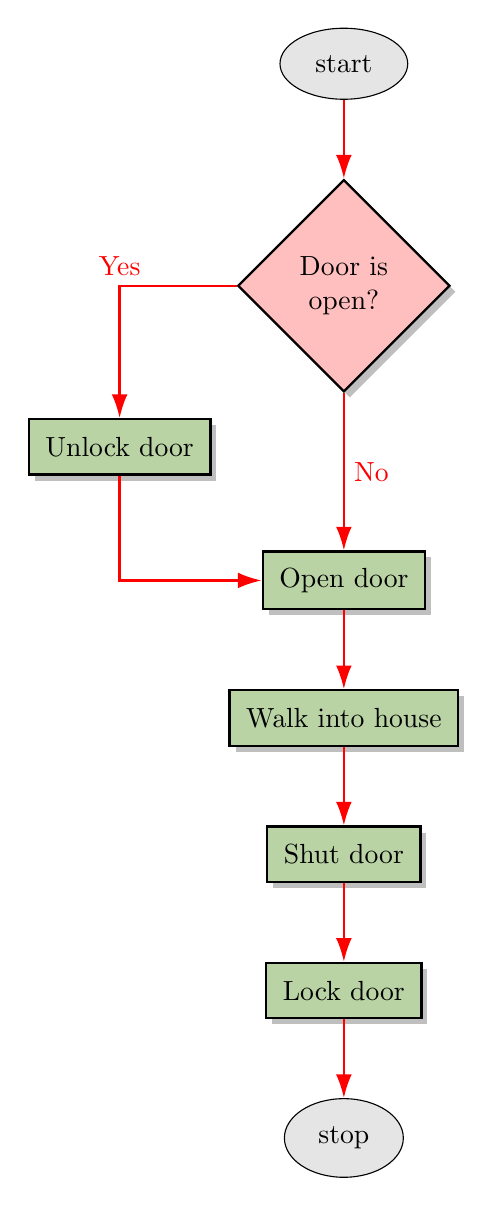
\begin{tikzpicture}[auto,
    -{Latex[length=3mm,width=2mm]},
    >=stealth
  ]
\node[st](start) {start};
\node[db, below=of start](0) {Door is \\ open?};
\node[jn, left=of 0](j1){};
\node[bb, below left=of 0](1) {Unlock door};
\node[bb, below= of 0, yshift=-1cm](2) {Open door};
\node[bb, below= of 2](3) {Walk into house};
\node[bb, below= of 3](4) {Shut door};
\node[bb, below= of 4](5) {Lock door};
\node[st, below=of 5](stop) {stop};
%\draw[-, Red, thick] (0) to (j1);
\draw[kcedge] (0) -| node[above]{Yes} (1);
\draw[kcedge] (1) |- (2);
\draw[kcedge] (0) to node[right]{No}(2);
\draw[kcedge] (2) to (3);
\draw[kcedge] (3) to (4);
\draw[kcedge] (4) to (5);
\draw[kcedge] (start) to (0);
\draw[kcedge] (5) to (stop);
  \end{tikzpicture}
}
\end{center}

\end{minipage}

\end{tabular}
\end{center}

\end{frame}
% frame end %%%%%%%%%%%%%%%%%%%%%%%%

\addtocounter{qnum}{1}
% frame begin %%%%%%%%%%%%%%%%%%%%%%%%
\begin{frame}[fragile]{Flowchart}
{If-Else Branch}

\textbf{PROBLEM \theqnum:} We have to affix postage stamp of the following denomination to the envelope:
\begin{itemize}
\item Rs. 30 for speed post
\item Rs. 35 for registered post
\end{itemize}

\begin{center}
\begin{tabular}{c @{\hspace{1cm}} c}
\begin{minipage}{0.4\textwidth}
\begin{lstlisting}[basicstyle=\ttfamily\scriptsize]
IF text T written on the
 given envelope E is 
 "SPEED POST" THEN
    Affix Rs. 30 stamp on E
ELSE IF text T written on
  E is "REGISTERED POST" THEN
    Affix Rs. 35 stamp on E
ENDIF
\end{lstlisting}
\end{minipage}
&
\begin{minipage}{0.45\textwidth}
\pause
\begin{center}
\resizebox{!}{0.5\textheight}{
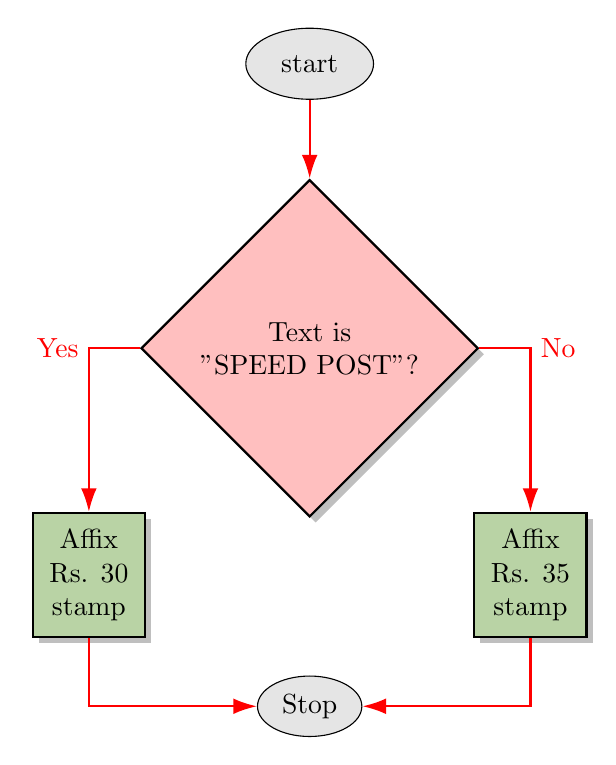
\begin{tikzpicture}[auto,
    -{Latex[length=3mm,width=2mm]},
    >=stealth
  ]
\node[st](start) {start};
\node[db, below=of start](0) {Text is \\ "SPEED POST"?};
\node[bb, below left=of 0](1) {Affix \\ Rs. 30 \\ stamp};
\node[bb, below right=of 0](2) {Affix \\ Rs. 35 \\ stamp};
\node[ellipse, draw=Black, fill=Gray!20, below= of 0, yshift=-1cm](stop) {Stop};

%\draw[-, Red, thick] (0) to (j1);
\draw[kcedge] (0) -| node[left]{Yes} (1);
\draw[kcedge] (0) -| node[right]{No}(2);
\draw[kcedge] (1) |- (stop);
\draw[kcedge] (2) |- (stop);
\draw[kcedge] (start) -- (0);
  \end{tikzpicture}
}
\end{center}

\end{minipage}

\end{tabular}
\end{center}

\end{frame}
% frame end %%%%%%%%%%%%%%%%%%%%%%%%

\addtocounter{qnum}{1}
% frame begin %%%%%%%%%%%%%%%%%%%%%%%%
\begin{frame}[fragile]{Flowchart}
{Loop}

\textbf{PROBLEM \theqnum:} You are in front of the door of your house. The door is already locked. Enter the house and lock the door from inside. Take one step at a time.

\begin{center}
\begin{tabular}{c @{\hspace{1cm}} c}
\begin{minipage}{0.4\textwidth}
\begin{lstlisting}[basicstyle=\ttfamily\scriptsize]
Unlock door
WHILE inside house is false THEN
  Take a step
DONE
Lock door
\end{lstlisting}
\end{minipage}
&
\begin{minipage}{0.45\textwidth}
\pause
\begin{center}
\resizebox{!}{0.6\textheight}{
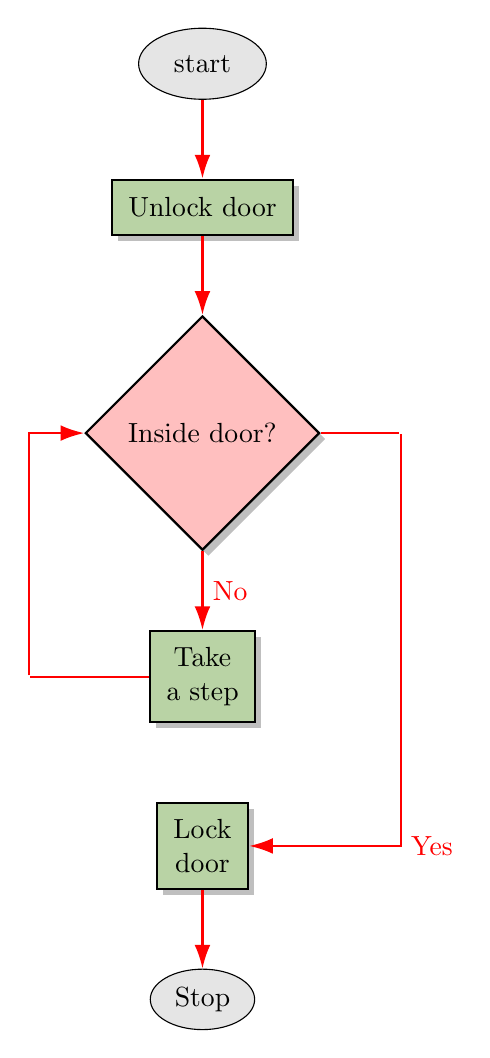
\begin{tikzpicture}[auto,
    -{Latex[length=3mm,width=2mm]},
  ]

\node[st](start) {start};
\node[bb, below=of start](i1) {Unlock door};
\node[db, below=of i1](0) {Inside door?};
\node[bb, below=of 0](1) {Take \\ a step};
\node[jn, left=1.5cm of 1] (j1){};
\node[jn, right=of 0] (j2){};
\node[bb, below =of 1](2) {Lock \\ door};
\node[ellipse, draw=Black, fill=Gray!20, below= of 2](3) {Stop};

\draw[kcedge] (start) -- (i1);
\draw[kcedge] (i1) -- (0);
\draw[-, Red, thick] (1) to (j1);
\draw[kcedge] (j1) |- (0);
\draw[kcedge] (0) to node[right]{No} (1);
\draw[-, Red, thick] (0) to (j2);
\draw[kcedge] (j2) |- node[right]{Yes}(2);
\draw[kcedge] (2) to (3);
  \end{tikzpicture}
}
\end{center}

\end{minipage}

\end{tabular}
\end{center}

\end{frame}
% frame end %%%%%%%%%%%%%%%%%%%%%%%%

\addtocounter{qnum}{1}
% frame begin %%%%%%%%%%%%%%%%%%%%%%%%
\begin{frame}[fragile]{Flowchart}
{If-Else if-Else Branch}
\textbf{PROBLEM \theqnum:} Program that takes two numbers and a choice (1 for addition, 2 for multiplication) and does appropriate calculation.

\begin{center}
\begin{tabular}{c @{\hspace{1cm}} c}
\begin{minipage}{0.4\textwidth}
\begin{lstlisting}[basicstyle=\ttfamily\scriptsize]
Input n1, n2, choice
IF choice = 1 THEN
  OUTPUT n1 + n2
ELSE IF choice = 2 THEN
  OUTPUT n1 * n2
ELSE
  OUTPUT "INVALID CHOICE."
\end{lstlisting}
\end{minipage}
&
\begin{minipage}{0.45\textwidth}
\pause
\begin{center}
\resizebox{!}{0.5\textheight}{
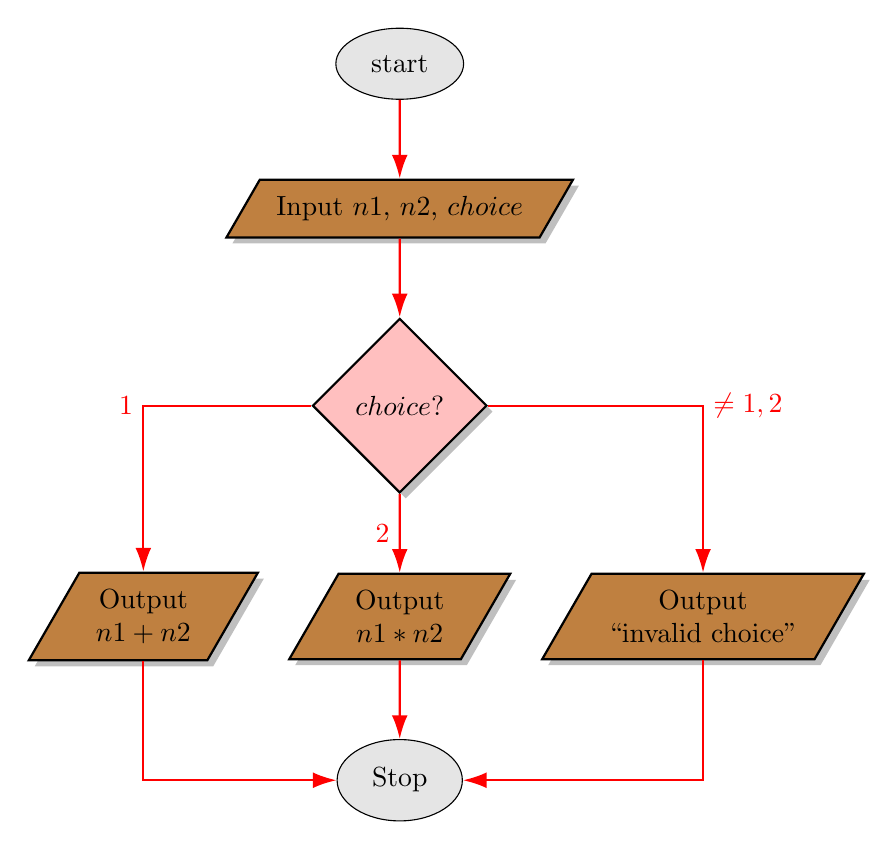
\begin{tikzpicture}[auto,
%    -{Latex[length=3mm,width=2mm]},
  ]

\node[st](start) {start};
\node[io, below=of start](in1) {Input $n1$, $n2$, $choice$};
\node[db, below=of in1](d1) {$choice?$};

\node[io, below=of d1](i2) {Output \\ $n1 * n2$};
\node[io, left=of i2](i1) {Output \\ $n1 + n2$};
\node[io, right=of i2](i3) {Output \\ ``invalid choice"};
\node[st, below=of i2](stop) {Stop};

\draw[kcedge] (start) -- (in1);
\draw[kcedge] (in1) -- (d1);
\draw[kcedge] (d1) -| node[left]{$1$}(i1);
\draw[kcedge] (d1) -- node[left]{$2$}(i2);
\draw[kcedge] (d1) -| node[right]{$\neq 1, 2$}(i3);
\draw[kcedge] (i1) |- (stop);
\draw[kcedge] (i2) to (stop);
\draw[kcedge] (i3) |- (stop);
  \end{tikzpicture}
}
\end{center}

\end{minipage}

\end{tabular}
\end{center}

\end{frame}
% frame end %%%%%%%%%%%%%%%%%%%%%%%%

% frame begin %%%%%%%%%%%%%%%%%%%%%%%%
\begin{frame}[fragile]{Flowchart}
{If-Else if-Else Branch}

\begin{center}
\begin{tabular}{c @{\hspace{0.5cm}$\equiv$\hspace{0.5cm}} c}
\begin{minipage}{0.45\textwidth}
\begin{center}
\resizebox{!}{0.5\textheight}{
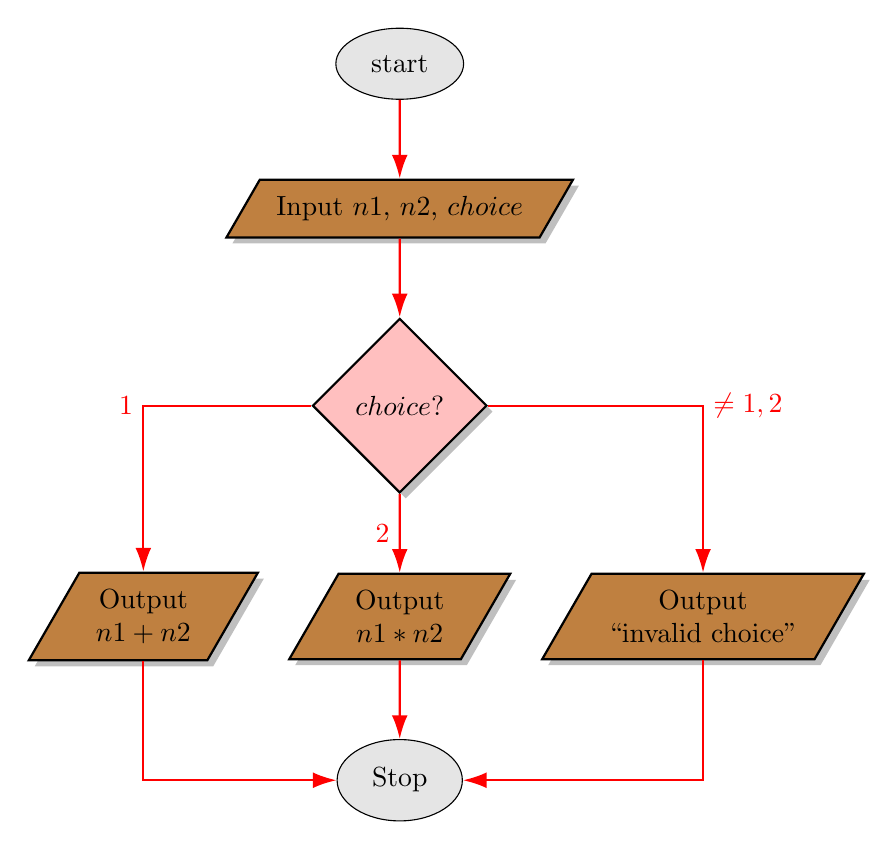
\begin{tikzpicture}[auto,
%    -{Latex[length=3mm,width=2mm]},
  ]

\node[st](start) {start};
\node[io, below=of start](in1) {Input $n1$, $n2$, $choice$};
\node[db, below=of in1](d1) {$choice?$};

\node[io, below=of d1](i2) {Output \\ $n1 * n2$};
\node[io, left=of i2](i1) {Output \\ $n1 + n2$};
\node[io, right=of i2](i3) {Output \\``invalid choice"};
\node[st, below=of i2](stop) {Stop};

\draw[kcedge] (start) -- (in1);
\draw[kcedge] (in1) -- (d1);
\draw[kcedge] (d1) -| node[left]{$1$}(i1);
\draw[kcedge] (d1) -- node[left]{$2$}(i2);
\draw[kcedge] (d1) -| node[right]{$\neq 1, 2$}(i3);
\draw[kcedge] (i1) |- (stop);
\draw[kcedge] (i2) to (stop);
\draw[kcedge] (i3) |- (stop);
  \end{tikzpicture}
}
\end{center}

\end{minipage}
&
\pause
\begin{minipage}{0.45\textwidth}
\begin{center}
\resizebox{!}{0.5\textheight}{
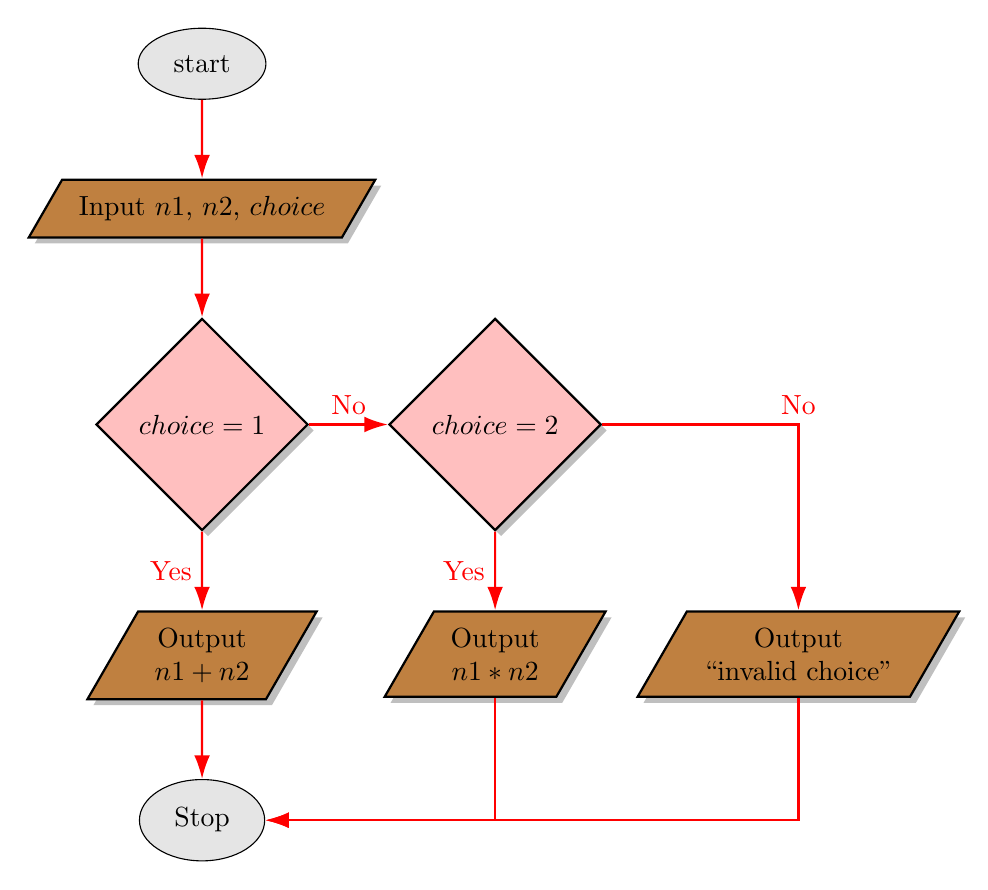
\begin{tikzpicture}[auto,
%    -{Latex[length=3mm,width=2mm]},
  ]

\node[st](start) {start};
\node[io, below=of start](in1) {Input $n1$, $n2$, $choice$};
\node[db, below=of in1](d1) {$choice=1$};
\node[db, right=of d1](d2) {$choice=2$};
%\node[db, right=of d2](d3) {$choice\neq 1,2$};

\node[io, below=of d1](i1) {Output \\ $n1 + n2$};
\node[io, below=of d2](i2) {Output \\ $n1 * n2$};
\node[io, right=of i2](i3) {Output \\ ``invalid choice"};
\node[st, below=of i1](stop) {Stop};

\draw[kcedge] (start) -- (in1);
\draw[kcedge] (in1) -- (d1);
\draw[kcedge] (d1) -- node[left]{Yes}(i1);
\draw[kcedge] (d1) -- node[above]{No}(d2);
\draw[kcedge] (d2) -- node[left]{Yes}(i2);
\draw[kcedge] (d2) -| node[above]{No}(i3);
% \draw[kcedge] (d3) -- node[right]{$\neq 1, 2$}(i3);
\draw[kcedge] (i1) -- (stop);
\draw[kcedge] (i2) |- (stop);
\draw[kcedge] (i3) |- (stop);
  \end{tikzpicture}
}
\end{center}

\end{minipage}

\end{tabular}
\end{center}

\end{frame}
% frame end %%%%%%%%%%%%%%%%%%%%%%%%

% frame begin %%%%%%%%%%%%%%%%%%%%%%%%
\begin{frame}[fragile]{Flowchart}
{Building Blocks}

\begin{center}
\begin{tabular}{|c|c|}
\hline
Instruction
&
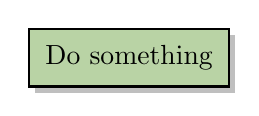
\begin{tikzpicture}
\node[bb]{Do something};
\end{tikzpicture}
\\
\hline
Decision
&

\begin{tikzpicture}
\node[db]{Check \\ condition};
\end{tikzpicture} \\
\hline

\end{tabular}
\end{center}

\end{frame}
% frame end %%%%%%%%%%%%%%%%%%%%%%%%

% frame begin %%%%%%%%%%%%%%%%%%%%%%%%
\begin{frame}[fragile]{Flowchart}
{Building Blocks}

\begin{center}
\begin{tabular}{|c|c|}
\hline
Input/Output
&
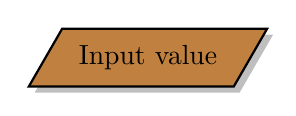
\begin{tikzpicture}
\node[io]{Input value};
\end{tikzpicture}
\\
\hline
Start/Stop
&
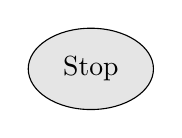
\begin{tikzpicture}
\node[st]{Stop};
\end{tikzpicture} \\
\hline

\end{tabular}
\end{center}

\end{frame}
% frame end %%%%%%%%%%%%%%%%%%%%%%%%


% frame begin %%%%%%%%%%%%%%%%%%%%%%%%
\begin{frame}[fragile]{Flowchart}
{Advantages}

\begin{enumerate}
\item It helps think about the algorithm/process in a pictorial way.
\item It's not a formal language like a programming language (e.g. Python). Therefore, doesn't get stuck due to syntax errors.
\end{enumerate}
\end{frame}
% frame end %%%%%%%%%%%%%%%%%%%%%%%%

\end{document}
